% Definição do tamanho da letra, folha e estilo.
\documentclass[12pt, a4paper]{article}

% Definição de pacotes.
%% Padrão UTF-8.
%% Texto brasileiro.
%% Identação dos parágrafos.
%% Adição de imagens.
%% Geometria da página de acordo com a ABNT.
\usepackage[utf8]{inputenc}
\usepackage[brazil]{babel}
\usepackage{indentfirst}
\usepackage{graphicx}
\usepackage{geometry}
\geometry{a4paper, left = 3cm, right = 3cm, top = 3cm, bottom = 3cm}

% Numeração da página.
\pagenumbering{arabic}

% Path das imagens.
\graphicspath{{./img/}}

\title{\textbf{Modificações no Processador Multi-ciclo}}
\author{
	Guimarães, João Guilherme M.\\
	\texttt{joaog95@live.com}
	\and
	Muniz, Lucas L. R.\\
	\texttt{lucaslc01@hotmail.com}
}
\date{\today}

\begin{document}
	% Escrever o título, autor e data.
	\maketitle
	
	% Espaçamento vertical
	\vspace{1cm}
	
	% Nova seção
	\section{Objetivo da prática}
	
	\par A nona aula prática da disciplina de Laboratório de Arquitetura de Computadores I, teve como objetivo realizar modificações no código do processador multi-ciclo desenvolvido na aula anterior, estas mudanças são:
	
	\begin{itemize}
		\item Os registradores no formato da instrução passam a ter 4 bits;

		\item Mudança na relação entre os registradores de cada instrução e

		\item Mudança no \textit{Opcode} de algumas instruções.
	\end{itemize}

    \section{Descrição das Atividades}

    \par O aumento de um bit de endereçamento no formato da instrução, permitiu que \textbf{RF} tivesse um acréscimo de 8 registradores, passando assim de 8 para 16, e para manter o padrão de projeto, o registrador referente ao \textbf{PC} também foi alterado, estando agora na posição 15, a última posição de \textbf{RF}.
    
    \vspace{\baselineskip}
    
    \par As alterações entre as relações dos registradores de cada instrução, acarretou na criação de uma nova variável de controle, \textit{WriteReg}, possibilitando com que as instruções possam salvar seus dados em um dos 3 registradores, \textbf{X}, \textbf{Y} e \textbf{Z}, sendo que antes, a utilização do registrador \textbf{X} era obrigatória.

    \vspace{\baselineskip}
    
    \par E por último, a mudança no \textit{Opcode} das instruções, acarretou em mudanças simples no código de teste e na estrutura do módulo de controle.

    \vspace{\baselineskip}

    \par A seguir um resumo das alterações:
    
    \begin{itemize}
		\item Expansão de \textbf{RF} de 8 para 16 registradores;

        \item Substituição do registrador referente ao \textbf{PC} para a posição 15;

        \item Criação da nova variável de controle \textit{WriteReg} e
        
        \item Correção dos \textit{Opcodes} das instruções.
    \end{itemize}

    \section{Simulação}
    
    \par Após as modificações necessárias, iniciamos a simulação utilizando a instrução \textit{copy input}, pois ela é responsável por inicializar os dados nos registradores, sendo assim, se torna presente nas simulações das demais instruções. Segue abaixo o código, a representação e a descrição breve da simulação.

    \vspace{\baselineskip}
    
    \begin{figure}[!h]
        \centering
        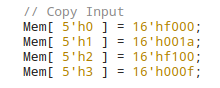
\includegraphics{./COPY_INPUT/copy_input_code}
        \caption{Código da simulação da instrução \textit{Copy Input}}
	    \label{fig: copy input code}
    \end{figure}

    \vspace{\baselineskip}

    \begin{figure}[!h]
    	\centering
        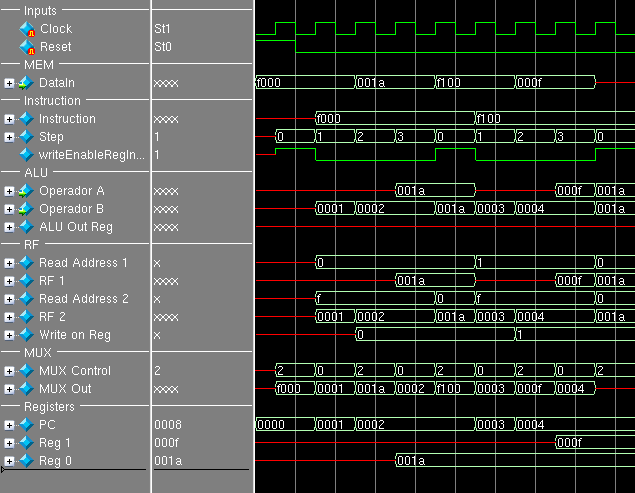
\includegraphics[width=15cm]{./COPY_INPUT/copy_input}
    	\caption{Simulação da instrução \textit{Copy Input}}
    	\label{fig: copy input}
    \end{figure}

    \par Baseando se na figura \ref{fig: copy input}, temos a esquerda as entradas \textit{Clock} e \textit{Reset}, e as variáveis necessárias para visualizar melhor o \textit{datapath} da instrução. A simulação consistiu em carregar da memória os dados \textit{001a} e \textit{000f} e salvá-los nos registradores \textit{0} e \textit{1}, respectivamente. O resultado da simulação ocorreu como esperado, já que no início do passo 3 de cada instrução, o registrador referente já estava escrito com o dado proposto.
    
    \vspace{\baselineskip}

    \par A segunda instrução a ser simulada é a \textit{not}, que consiste em realizar os mesmos procedimentos descritos na figura \ref{fig: copy input code} para inicializar os registradores \textit{0} e \textit{1}, com acréscimo de inverter o dado no registrador \textbf{X} e armazena-lo no registrador \textbf{Y}.
    
    \begin{figure}[!h]
        \centering
        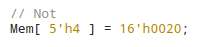
\includegraphics{./NOT/not_code}
        \caption{Código da simulação da instrução \textit{Not}}
        \label{fig: not code}
    \end{figure}

    \vspace{\baselineskip}

    \begin{figure}[!h]
        \centering
        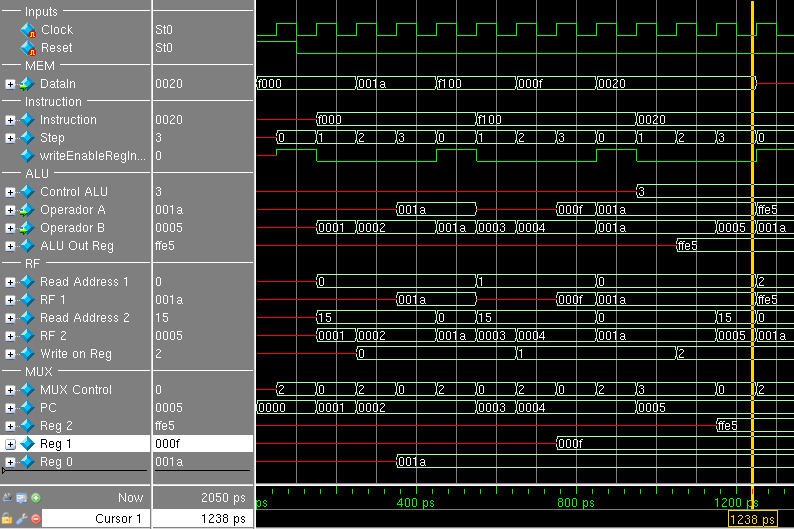
\includegraphics[width=15cm]{./NOT/not}
        \caption{Simulação da instrução \textit{Not}}
        \label{fig: not}
    \end{figure}

    \par Como pode ser visto na figura \ref{fig: not}, o resultado obtido foi igual ao esperado, já que no terceiro passo da instrução \textit{000f}, ocorreu a escrita no registrador \textit{2}.
    
    \vspace{\baselineskip}
    
    \par A última simulação descrita neste relatório, será a da instrução \textit{store}, que novamente consiste em realizar os procedimentos descritos na figura \ref{fig: copy input code} para inicializar os registradores e posteriormente, salvar na memória de endereço \textit{11010 (001a)} o dado \textit{000f}.
    
    \begin{figure}[!h]
    	\centering
    	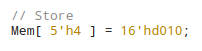
\includegraphics{./STORE/store_code}
    	\caption{Código da simulação da instrução \textit{Store}}
    	\label{fig: store code}
    \end{figure}
    
    \vspace{\baselineskip}
    
    \begin{figure}[!h]
    	\centering
    	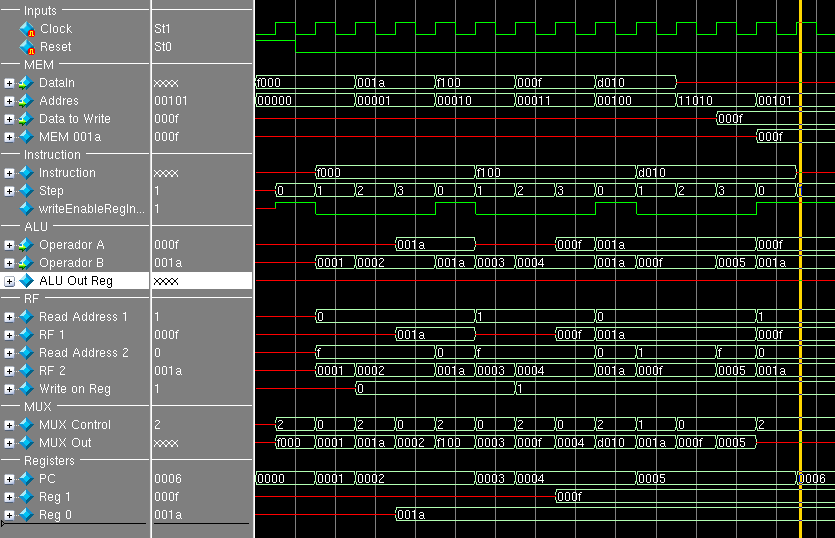
\includegraphics[width=15cm]{./STORE/store}
    	\caption{Simulação da instrução \textit{Store}}
    	\label{fig: store}
    \end{figure}

    \par Baseando se na figura \ref{fig: store}, é possível perceber que a instrução \textit{store} diferente das demais, tem o seu resultado obtido somente no passo 0 da próxima instrução, que foi de acordo com o esperado.
    
    \vspace{\baselineskip}
    
    \par \noindent Obs.: o código e a simulação do restante das instruções se encontram na pasta do projeto, mais especificamente, na pasta simulação.
	
	\section{Dificuldades}
	
	\par As principais dificuldades obtidas no desenvolvimento desta prática foram:
	
	\begin{enumerate}
		\item Encontrar e resolver o erro na instrução \textit{conditional copy}, já que a mesma realizava o inverso do proposto (executava o processo de \textit{copy} somente quando o valor na \textbf{ULA} era diferente de 0) e

        \item Realizar os testes de cada instrução após as alterações, o que resulta em um total de 9 simulações.
	\end{enumerate}

	\section{Conclusão}
	
	\par Com a execução desta prática, pudemos aperfeiçoar nossos conhecimentos em projetos de processadores multi-ciclos e da linguagem Verilog, além de exercitar o trabalho em equipe.

\end{document}
	